\documentclass[border=0cm]{standalone}
\usepackage{xcolor}
\usepackage{tikz}
\usetikzlibrary{arrows, arrows.meta}
\tikzset{    
    barbarrow/.style={ % style that just defines the arrow tip
        >={Straight Barb[left,length=5pt,width=5pt]},
        thick,
        <->
    },
    blues/.style={
        color=blue
    },
    reds/.style={
        color=red
    }
}
\definecolor{light-gray}{gray}{0.975}
\definecolor{pcolor}{rgb}{0.21, 0.27, 0.31}
\definecolor{purple}{rgb}{1.0, 0.0 1.0}
\begin{document}
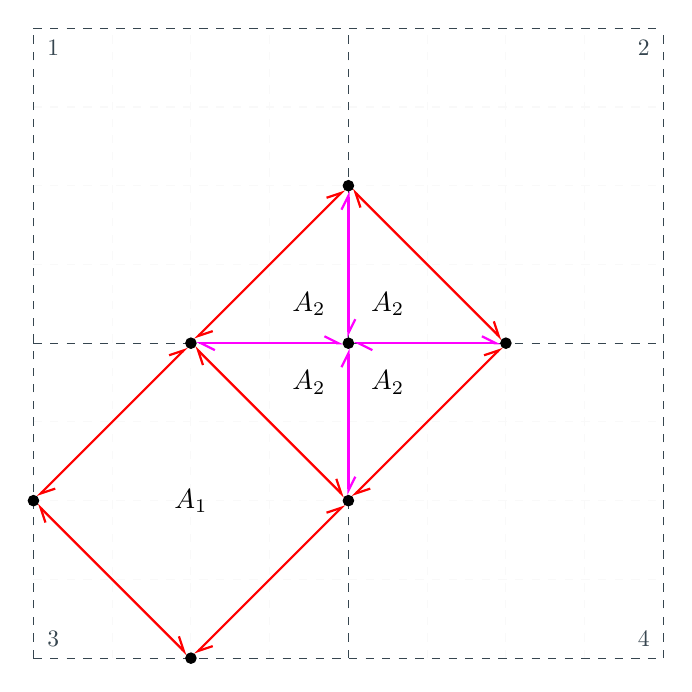
\begin{tikzpicture}
    \tikzstyle{node1}=[draw,scale=0.4,shape=circle,color=black,fill=black]
    \tikzstyle{node2}=[draw,scale=0.4,shape=circle,color=red,fill=red]
    \tikzstyle{text}=[draw,scale=0.5,color=black]
    \draw[color=light-gray, style=dashed] (0,0) grid (8,8);
    \draw[color=pcolor, style=dashed, step=4] (0,0) grid (8,8);
    \node[scale=0.85, color = pcolor] at (0.25, 7.75) {$1$};
    \node[scale=0.85, color = pcolor] at (7.75, 7.75) {$2$};
    \node[scale=0.85, color = pcolor] at (0.25, 0.25) {$3$};
    \node[scale=0.85, color = pcolor] at (7.75, 0.25) {$4$};

    \node[node1] (A) at (0,2) {};
    \node[node1] (C) at (2,0) {};
    \node[node1] (E) at (2,4) {};
    \node[node1] (K) at (4,2) {};
    \node[node1] (M) at (4,6) {};
    \node[node1] (R) at (6,4) {};
    \node[node1] (Z) at (4,4) {};
    \node at (2,2) {$A_1$};
    \node at (3.5,4.5) {$A_2$};
    \node at (4.5,4.5) {$A_2$};
    \node at (3.5,3.5) {$A_2$};
    \node at (4.5,3.5) {$A_2$};
    
    \draw[barbarrow, color=red] (A) -- (C); %\draw[barbarrow, color=red] (C.155) -- (A.-65);
    \draw[barbarrow, color=red] (A) -- (E); %\draw[barbarrow, color=red] (E.-155) -- (A.25); 
    \draw[barbarrow, color=red] (C) -- (K); %\draw[barbarrow, color=red] (K.-115) -- (C.25); 
    \draw[barbarrow, color=red] (E) -- (K); %\draw[barbarrow, color=red] (K.155) -- (E.-65); 
    \draw[barbarrow, color=red] (E) -- (M); 
    \draw[barbarrow, color=red] (K) -- (R); 
    \draw[barbarrow, color=red] (M) -- (R);
    \draw[barbarrow, color=purple] (Z) -- (E); %\draw[barbarrow, color=red] (E.20) -- (Z.160);
    \draw[barbarrow, color=purple] (Z) -- (R); %\draw[barbarrow, color=red] (R.200) -- (Z.-20);
    \draw[barbarrow, color=purple] (Z) -- (M); %\draw[barbarrow, color=red] (M.-70) -- (Z.70);
    \draw[barbarrow, color=purple] (Z) -- (K); %\draw[barbarrow, color=red] (K.110) -- (Z.-110);
\end{tikzpicture}
\end{document}
